\newpage
\subsubsection{UC7.1 - Gestione Proprio Profilo Utente}
\label{UC7.1}

\begin{figure}[ht]
	\centering
	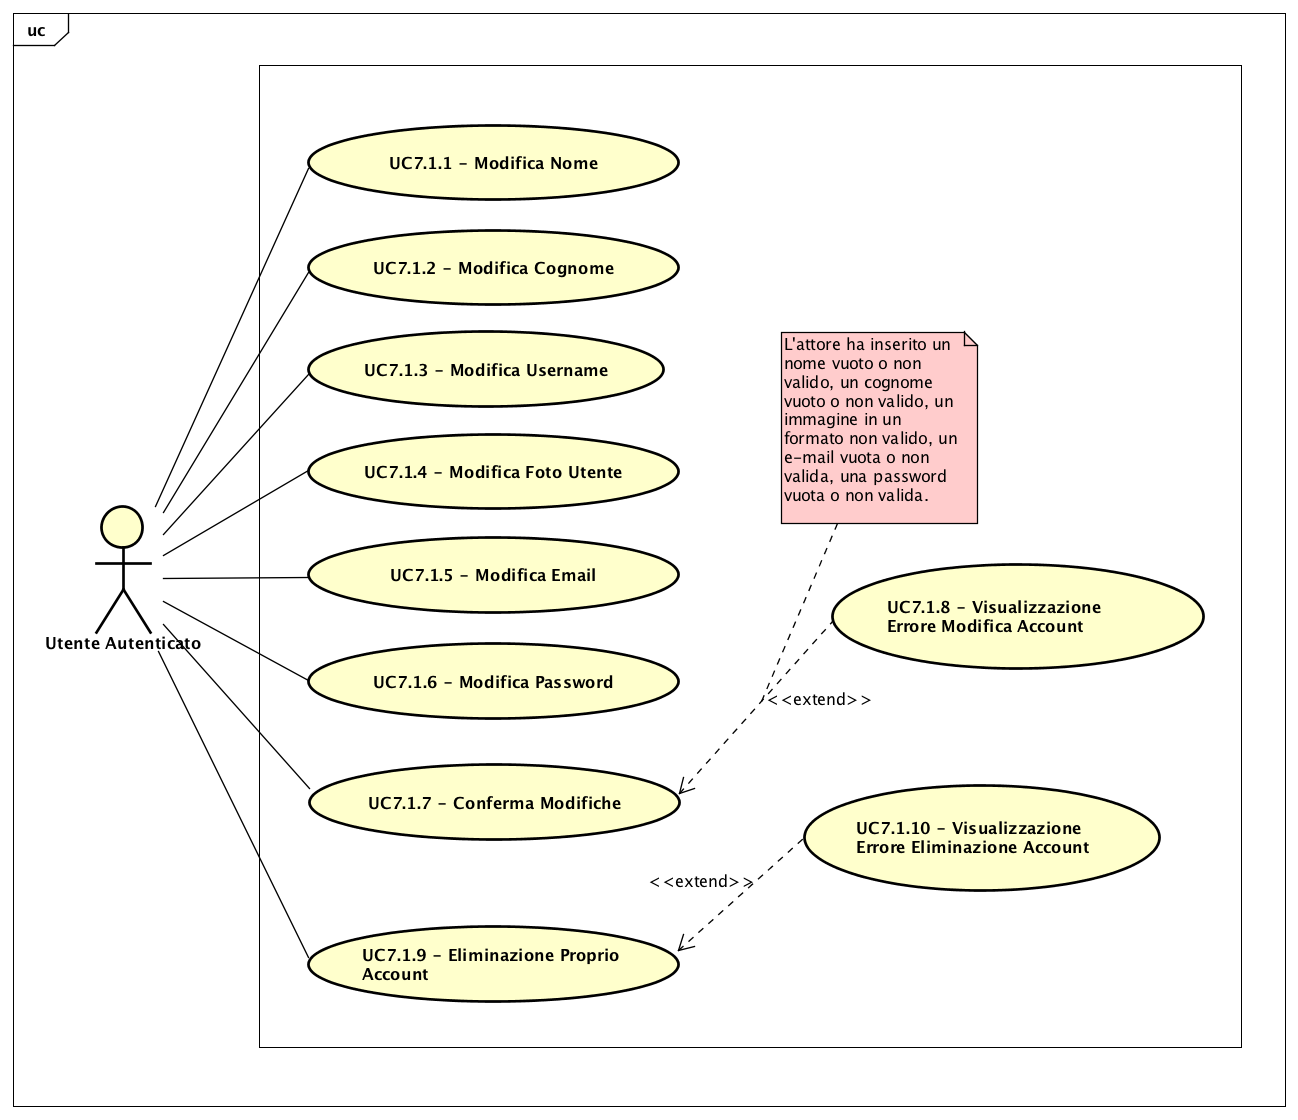
\includegraphics[scale=0.45]{UML/UC7_1.png}
	\caption{UC7.1 - Gestione Proprio Profilo Utente}
\end{figure}
\FloatBarrier
\begin{longtable}{ l | p{11cm}}
	\hline
	\rowcolor{Gray}
	 \multicolumn{2}{c}{UC7.1 - Gestione Proprio Profilo Utente} \\
	 \hline
	 \textbf{Attori} & Utente autenticato  \\
	\textbf{Descrizione} & L’utente pu\'{o} modificare le proprie informazioni personali  \\
	\textbf{Pre-Condizioni} & L’Utente \`{e} nel proprio profilo \\
	\textbf{Post-Condizioni} & L’Utente ha aggiornato il proprio profilo \\
	\textbf{Scenario Principale} & 
	\begin{enumerate*}[label=(\arabic*.),itemjoin={\newline}]
		\item L'utente pu\`{o} modificare il Nome (UC7.1.1)
		\item L'utente pu\`{o} modificare il Cognome (UC7.1.2)
		\item L'utente pu\`{o} modificare l'Username (UC7.1.3)
		\item L'utente pu\`{o} modificare la Foto Utente (UC7.1.4)
		\item L'utente pu\`{o} modificare l'Email (UC7.1.5)
		\item L'utente pu\`{o} modificare la Password (UC7.1.6)
		\item L'utente pu\`{o} confermare le Proprie Modifiche (UC7.1.7)
		\item L'utente pu\`{o} eliminare il Proprio Account (UC7.1.9)
	\end{enumerate*}\\
	\textbf{Scenari Alternativi} & 
		\begin{enumerate*}[label=(\arabic*.),itemjoin={\newline}]
		\item L'utente visualizza un Errore di Modifica Account se le modifiche risultano illegali (UC7.1.8)
		\item L'utente visualizza un Errore di Modifica Account se risulta un errore durante eliminazione (UC7.1.10)
	\end{enumerate*}\\
\end{longtable}



